\section{Specific requirements}
	\subsection{External interface requirements}
		\subsubsection{User Interfaces: Web Page}
		In this section is presented a minimal mock-up of the web and mobile interfaces on both users and taxis side. 
		
		These have to be considered as an example of what at least is needed in the interface and don't are final version of the product.
		\paragraph{Index}
		\begin{center}
			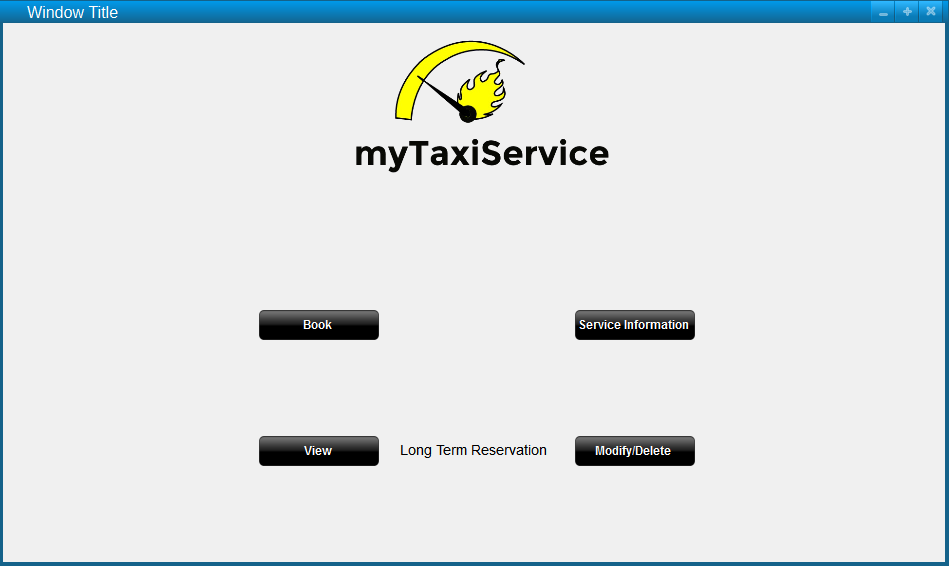
\includegraphics[width=0.90\textwidth]{./images/index}
		\end{center}
		\paragraph{Book a Taxi}
		\begin{center}
			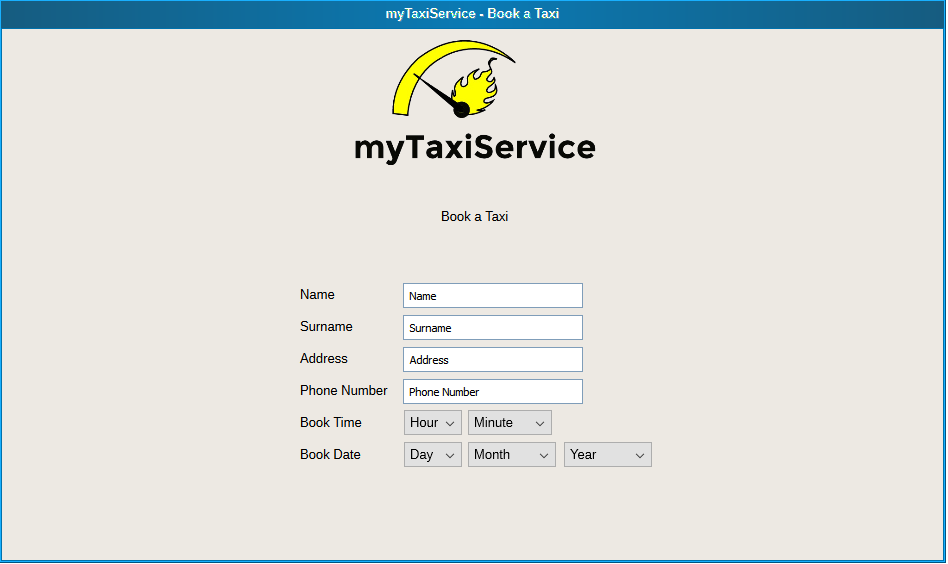
\includegraphics[width=0.90\textwidth]{./images/check_reservation}
		\end{center}
		\paragraph{View/Modify/Delete a Long Term Reservation}
		\begin{center}
			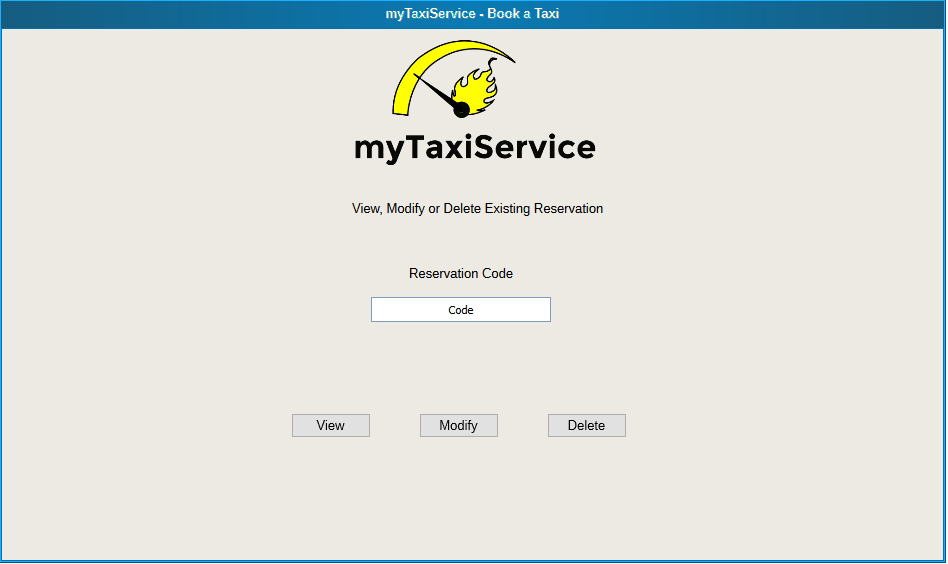
\includegraphics[width=0.90\textwidth]{./images/modify_delete_reservation}
		\end{center}
		\paragraph{Who We Are}
		\begin{center}
			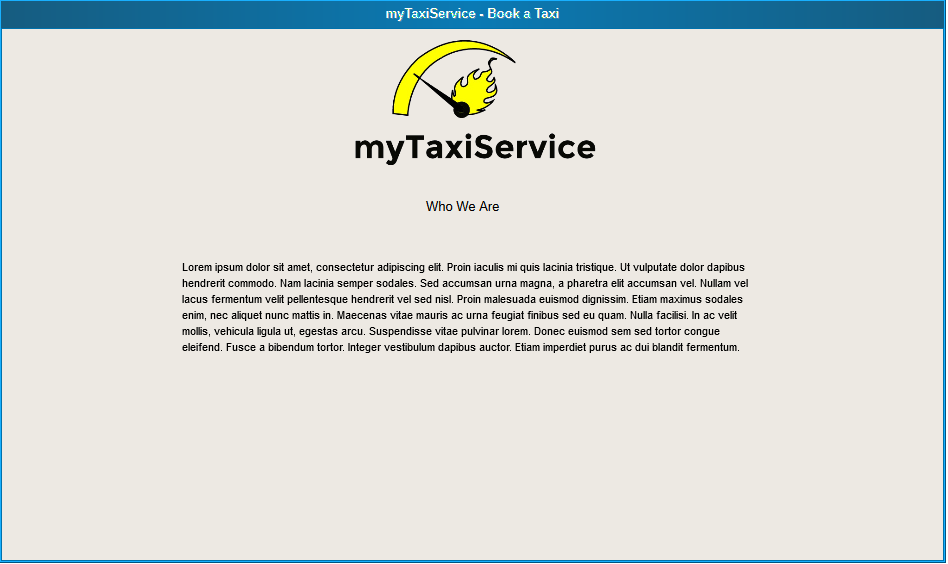
\includegraphics[width=0.90\textwidth]{./images/who_we_are}
		\end{center}
		
		\subsubsection{User Interfaces: Mobile Application}
		\paragraph{Home Page}
		\begin{center}
		    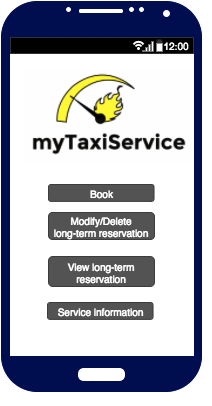
\includegraphics[width=0.32\textwidth]{./images/TELEFONO1User}
		\end{center}
		\paragraph{Booking}
		\begin{center}
		    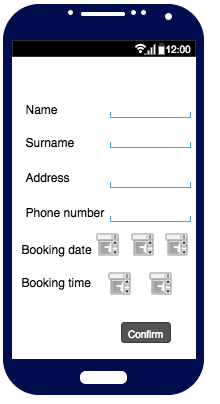
\includegraphics[width=0.35\textwidth]{./images/TELEFONO2User}
		\end{center}
		\paragraph{Insertion of the long-term reservation code}
		\begin{center}
		    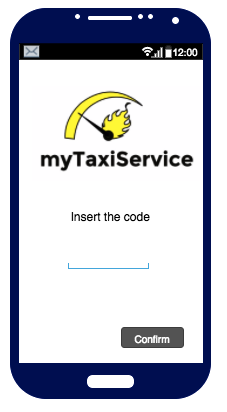
\includegraphics[width=0.35\textwidth]{./images/TELEFONO3User}
		\end{center}
		\paragraph{Choosing of long-term reservation modification or elimination}
		\begin{center}
		    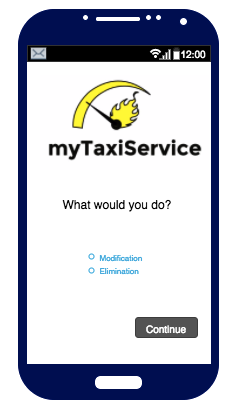
\includegraphics[width=0.35\textwidth]{./images/TELEFONO4User}
		\end{center}
		\paragraph{Choosing of new long-term reservation date and time}
		\begin{center}
		    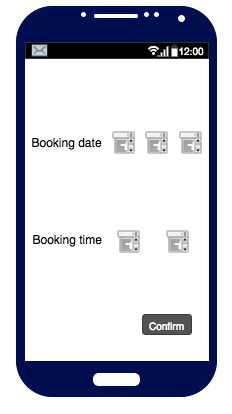
\includegraphics[width=0.35\textwidth]{./images/TELEFONO5User}
		\end{center}
		\paragraph{Service Informations}
		\begin{center}
		    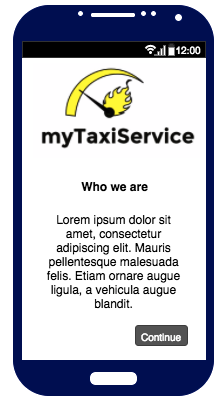
\includegraphics[width=0.35\textwidth]{./images/TELEFONO6User}
		\end{center}
		
		
		\subsubsection{Taxi Interfaces: Mobile Application}
		\paragraph{First Page}
		\begin{center}
		    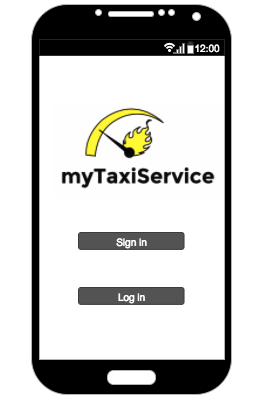
\includegraphics[width=0.40\textwidth]{./images/TELEFONO1}
		\end{center}
		\paragraph{Registration Page}
		\begin{center}
		    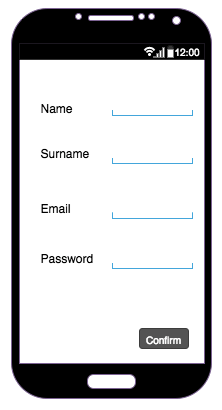
\includegraphics[width=0.35\textwidth]{./images/TELEFONO2}
		\end{center}
		\paragraph{Login}
		\begin{center}
		    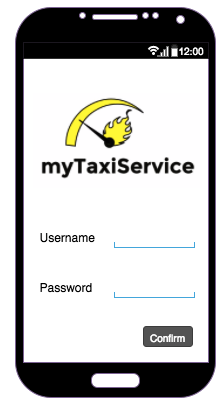
\includegraphics[width=0.35\textwidth]{./images/TELEFONO3}
		\end{center}
		\paragraph{Home Page}
		\begin{center}
		    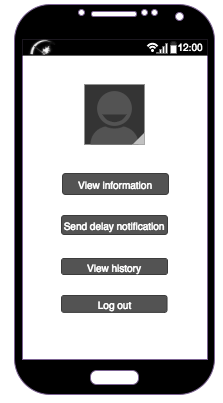
\includegraphics[width=0.35\textwidth]{./images/TELEFONO4}
		\end{center}
		\paragraph{View Information About The Current Ride}
		\begin{center}
		    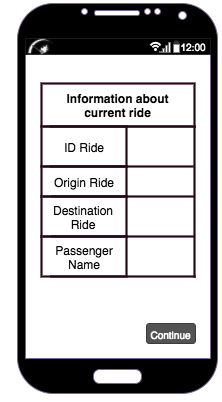
\includegraphics[width=0.32\textwidth]{./images/TELEFONO5}
		\end{center}
		\paragraph{View Information About The Previous Rides}
		\begin{center}
		    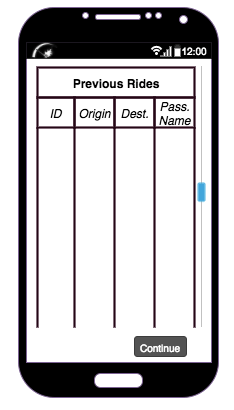
\includegraphics[width=0.35\textwidth]{./images/TELEFONO6}
		\end{center}
		\paragraph{Service Confirmation/Rejection}
		\begin{center}
		    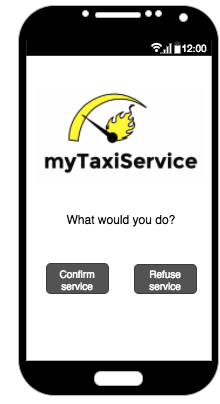
\includegraphics[width=0.32\textwidth]{./images/TELEFONO7}
		\end{center}
		
		\subsubsection{Hardware interfaces}
			There is the necessity to have:
			\begin{itemize}
				\item a machine dedicated to database-server, capable to manage high-volume transactions;
				\item a machine to run the main software and the web-interface;
				\item a private redundant gigabit network connecting both machines;
				\item a public redundant connection to internet for the web-server machine, with adequate speed and scalable traffic quota.
			\end{itemize}
			Hardware can be purchased or rented as virtual-server or cloud. In any case, the server must be colocated to appropiate server farm to guarantee safety and security.
		\subsubsection{Software interfaces}
			There is the necessity to have:
			\begin{itemize}
				\item a web server to provide information to browsers and mobile apps;
				\item the webserver must be capable to run PHP scripts;
				\item a DBMS, compatible with PHP, to store all the data managed by the system.
			\end{itemize}
		\subsubsection{Communication interfaces}
			The system will use the API, supplied by the external provider, being able to send SMS, as notifications, to the user. 
		\subsection{Functional Requirements}
		\subsubsection{Booking a Taxi ride}
		\begin{itemize}
			\item First of all, the system checks the date and the hour of the reservation. 
			\item In case of long-term reservation:
		\begin{enumerate}
			\item the system produces an alphanumeric code;
			\item the system stores this code, with name and surname of the user, in the relative database;
			\item the system assigns this code to the user.
		\end{enumerate}
			\item In case of short-term reservation:
		\begin{enumerate}
			\item the system checks what is the address inserted by the user;
			\item the system checks in which zone of the city is that address, using the GPS information;
			\item the system controls the taxis queue of that zone;
			\item if the taxis queue contains at least the identifier of one taxi:
				\begin{itemize}
					\item the system sends a notification to the first taxi driver of the queue;
					\item when it will receive the confirm, the system tells the user that the reservation is been realized;
				\end{itemize}	  
			\item if the taxis queue hasn't got any taxis identifiers:
				\begin{itemize}
					\item the system checks the queue of the four adjacent zones of that area;
					\item the system continues in this way as long as it finds an available taxi and then it will do the same things of the previous point;
					\item when the system will receive the confirm, it tells the user that there will be a delay;
					\item if the user decides to accept, the system tells him/her that the reservation is been realized, otherwise not.
				\end{itemize}
		\end{enumerate}
		\end{itemize}
		\subsubsection{Update a long-term reservation}
		\begin{itemize}
			\item The system receives the alphanumeric code from the user.
			\item The system checks the DB of the users.
			\item The system displays the information, collected from the DB, to the user.
			\item The system receives the modifications.
			\item The system saves the changed information in the DB.
			\item The system confirms to the user the modifications.
		\end{itemize}
		\subsubsection{Delete a long-term reservation}
		\begin{itemize}
			\item The system receives the alphanumeric code from the user.
			\item The system checks the DB of the users.
			\item The system deletes the found information.
			\item The system confirms to the user the correct elimination.
		\end{itemize}
		\subsubsection{Locate the Users}
		\begin{itemize}
			\item The system takes the address, inserted by the user.
			\item The system searches in which zone of the city is that address.
		\end{itemize}		
		\subsubsection{Managing Taxis location}
		\begin{itemize}
			\item The system uses the GPS informations.
			\item The system locates the position of all the taxis in the city.
			\item The system saves these information in the database and updates them every 2 minutes.
		\end{itemize}
		\subsubsection{Managing Taxi queue}
		\begin{itemize}
			\item Only in the case that a taxi is available, the system inserts its identifier in the zone queue, that is unique.
			\item If there is a new ride, the system chooses the first taxi in the queue, so, using a FIFO policy.
			\item If there is a new ride, but the interested zone queue is empty, the system checks the queues of the four adjacent zones; the system continues in this way as long as it finds an available taxi.
		\end{itemize}
		\subsubsection{Allow Taxi to register in the system}
		\begin{itemize}
			\item The system stores the data inserted by the Taxi Not Yet Registered.
			\item The system lets the Taxi to log in, using the vehicle plate and the password, inserted during the registration.
		\end{itemize}
		\subsubsection{Notify the users about their booking, their long-term reservation modification or elimination and about possible delays of the taxi}
		\begin{itemize}
			\item After a user's booking, the system sends to him, via SMS, a notification of the occurred booking. 
			\item After a long-term reservation modification, made by the user, the system sends to him, via SMS, a notification of the occurred modification.
			\item After a long-term reservation elimination, made by the user, the system sends to him, via SMS, a notification of the occurred elimination.
			\item After receiving from a Taxi a delay notification, the system sends to the user, via SMS, a notification of the Taxi delay.
		\end{itemize}
		\subsubsection{Notify Taxis about new available rides}
		\begin{itemize}
			\item The system sends to the first Taxi in the zone queue a notification of the new ride.
			\item If the Taxi answers the system with a negative reply, it sends another notification to the next Taxi of the zone queue; the system continues in this way as long as it finds an available taxi. 
		\end{itemize}
		\subsection{The World and the Machine}
		\begin{center}
			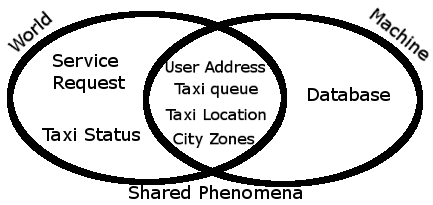
\includegraphics[width=0.85\textwidth]{./images/ellissi}
		\end{center}
		Service request and Taxi status are events that happen in the physical world; the machine then uses the data coming from the world to build a representation of it using taxi queue, taxi location and city zones. The database is only stored in the machine and contains all the data about users to send notification, long term reservations and data about taxis.
	\subsection{Scenarios}
		\subsubsection{Scenario 1}
		Bob has a meeting in Los Angeles the day after tomorrow. Since he hasn't a car, he decides to use myTaxiService and therefore rent a taxi to go to the airport. He grabs his cell phone and, with the mobile application of the service, he books a taxi. The app asks him his name, his surname, his phone number and the address where he wants to wait for the taxi. He inserts all the data requested and, after the server has stored these information in the database, with a SMS, it notifies Bob that the long-term reservation has been realized correctly. 
		The chosen day, ten minutes before the appointment, the system calls the first available taxi, searching it in the taxis queue of the zone in which there is the address specified by Bob. Unfortunately the first taxi doesn't answer the call; so the system puts him at the end of the queue and it calls the second taxi of the queue, which accepts the assignment. Then, Bob receives from the system, via SMS, a notification in which it was clarified that a taxi was coming to drive him to his destination.
		
		\subsubsection{Scenario 2}
		Today Francois starts his new job as a taxi driver. Yesterday morning, he signed up himself in myTaxiService application. Through his smart phone, he inserted only four information: his name, his surname, his email address and finally a password which he will use to sign in. After that, the system assigned him an alphanumeric code, that was the register of the taxi, which he will drive.
		During this morning, Francois signs in, inserting the username, that is the register of his taxi, and the password that he choose yesterday, during the registration. Clicking on the "Confirm" button, he accesses in the homepage of the mobile application. Francois has many possibilities to choose: he can view information about the current ride; he can view all the rides that he did in the past; he can send notifications of delay to the system and finally he can log out, of course at the end of the business day.
		While he is browsing the mobile application, Francois receives from the system a notification of a new ride. After the opening of this notification, Francois confirms the service and his business day starts.  
		
		\subsubsection{Scenario 3}
		Carl wants to go to visit one of his friends. Using the smart phone, he accesses to myTaxiService mobile application and he books a taxi, inserting name surname phone number and address, in the relative forms. The system stores these information in the database and then it checks in which zone there is the address specified by Carl. After that, the system notifies the first taxi in that zone's queue. The taxi receives a notification about that service by the system and he confirms the job, through the mobile application installed on his own smart phone. 
		Unfortunately a taxi's tyre runs flat; so the taxi driver sends a delay notification to the system, informing it that he can't complete the job. After the receive of this notification, therefore, the system puts that taxi at the end of the queue and it calls the second one that accepts the assignment. The system advises Carl, via SMS, that there will be a little delay.
		
		\subsubsection{Scenario 4}
		Thanks to one of his closest friends, Tizio has known a service, called MyTaxiService, that lets to book a taxi, through the web application or the user-friendly mobile one.
		Whereas his computer was broken, using his smart phone, first of all, Tizio has inserted his personal data, that were name, surname, phone number and home address. In that moment, the system has received the request of Tizio and it has checked in what zone of the city Tizio was asking for the service. In the taxis queue of that area, the system could have verify that there were no taxis. So it has become to check, starting from the zones near the area in which Tizio has requested a taxi, all the lists of available taxis. 
		Finally the system has found the only one taxi which, in that moment, was available. So the system has sent to Caio the notification of the new route. Besides Caio was standing, with his taxi, in a zone far from the place in which there was Tizio, he has confirmed the service, using the mobile application of his smart phone. After receiving the confirmation, the system has warned Tizio that the taxi would be arrived with a delay.
		About one hour later, Tizio is get into the Caio car and so, in a short time, he is arrived in the place where he would have meet his girlfriend Sempronia, relaxing himself, discovering that she was late more than him.
		
		\subsubsection{Scenario 5}
		Ann receives a call from one of her friend that tells her that her best friend has given birth to her son, Jimmy. Ann, due to the trains' strike decides to call myTaxiService to take her to the hospital to visit the newborn. So from her pc, she opens the web site of myTaxiService, that is www.mytaxiservice.com, clicks on the "Book" button to rent a taxi, after she has inserted all the needed data, that were name, surname, phone number and address, the system checks the taxis queue of the zone in which there is the address of Ann. Discovering that there is no available taxi in that zone in this specific time, the system searches for an available taxi in the queue of the adjacent zones. After it finds a free taxi in a nearby zone, the system notifies Ann, via SMS, that her reservation has been realized correctly but the taxi will arrive to Ann's address with a little delay. 
		
		\subsubsection{Scenario 6}
		Finally, today, Rossana would have taken the airplane. The flight was booked three days ago, but, because of bad weather, it was been deleted. So, she has accessed to the website of MyTaxiService to modify her reservation. She has used her notebook and then she has gone to the web page, concerning the modification/elimination of reservations. In the dedicated form, she has inserted the code that the system gave her to do this stuff, if she would have needed, but she could do it only until 15 minutes before the stipulated time. So she has postponed the reservation, without any problems.
		One hour before the meeting with the taxi, she has received a call from her boyfriend Heric, who wasn't really enthusiastic about her decision to go to USA for the Erasmus. When he has known that Rossana hasn't left yet, Heric has decided to give her a ride to the airport. So the girl, for that moment using her smart phone (the computer was in the luggage), has accessed to the mobile application of MyTaxiService to delete definitely her reservation. Going again in the dedicated page and then inserting her code in the specific form (but now choosing the "Elimination"), she has confirmed the cancellation of the reservation. 
	\newpage
	\subsection{UML Models}
		\subsubsection{Use Case}
			\paragraph{Registration of a new taxi driver}
			\begin{center}
			~\\
			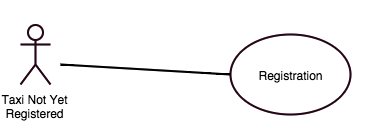
\includegraphics[width=0.60\textwidth]{./images/UseCaseTaxiNotYetRegistered.png}~
			\end{center}
			\begin{tabular}{l l}
		 \textbf {Name} & Registration  \\ \hline
		 \textbf{Actors} & Taxi not yet registered \\ \hline
		 \textbf{Entry conditions} & No entry conditions \\ \hline
		 \textbf{Event flow} & 
		 \parbox{0.7\textwidth}{
		 \begin{enumerate}
		 \item The new taxi driver not yet registered
		    \begin{itemize}
		    \item opens the myTaxiService mobile application;
		    \item clicks on "Sign In" link;
		    \item inserts name, surname, email address and a password for the login, after the opening of a new window;
		    \item clicks on "Confirm" link;
		    \end{itemize}
		 \item the system assigns an identifier, that is the taxi plate of the new taxi and which will be used by the new taxi driver as his username for the login.
		 \end{enumerate}
		 } \\ \hline
		 \textbf{Exit Condition} &  \parbox{0.7\textwidth}{The system adds the new taxi driver in the database and it grants him access to the application.} \\ \hline
		 \textbf{Exceptions} & Password inserted wrongly.
		\end{tabular}
		
		\newpage
		\paragraph{User side}
			\begin{center}
			~\\
		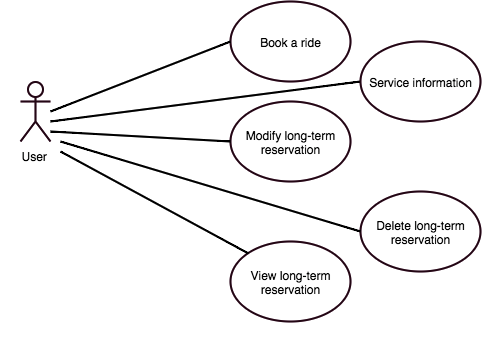
\includegraphics[width=0.90\textwidth]{./images/UseCaseUser.png}~
			\end{center}
		\newpage
		\subparagraph{Booking a ride}
		~\\[0.2cm]
			\vspace{20pt}
		\noindent
		
		\begin{tabular}{l l}
		 \textbf {Name} & Book a short-term reservation  \\ \hline
		 \textbf{Actors} & User, Taxi \\ \hline
		 \textbf{Entry conditions} & No entry conditions \\ \hline
		 \textbf{Event flow} & 
		 \parbox{0.7\textwidth}{
		 \begin{enumerate}
		 \item The user accesses to the web site or the mobile application.
		 \item The user clicks on "Book a ride".
		 \item The user inserts name, surname, phone number and address.
		 \item The user clicks on the "Confirm" button.
		 \item The system inserts the data of the user in the database.
		 \item The system identifies the area in which the address specified by the user is.
		 \item The system selects the first available taxi from the taxis queue.
		 \item The system sends the notification to the taxi.
		 \item The system sends a confirmation via SMS to the user.
		 \end{enumerate}
		 } \\ \hline
		 \textbf{Exit Condition} & \parbox{0.7\textwidth}{ The system adds the user information in the database.}\\ \hline
		 \textbf{Exceptions} & Address inserted wrongly.
		\end{tabular}
		
		\begin{tabular}{l l}
		 \textbf {Name} & Book a long-term reservation  \\ \hline
		 \textbf{Actors} & User, Taxi \\ \hline
		 \textbf{Entry conditions} & No entry conditions \\ \hline
		 \textbf{Event flow} & 
		 \parbox{0.7\textwidth}{
		 \begin{enumerate}
		 \item The user accesses to the web site or the mobile application.
		 \item The user clicks on "Book a ride".
		 \item The user inserts name, surname, phone number and address.
		 \item The user specifies the date and the hour of the long-term reservation.
		 \item The user clicks on the "Confirm" button.
		 \item If the date is the actual one, the system checks if the current time is at least two hours before the long-term reservation time.
		 \item The system inserts the data of the user in the database.
		  \item The system sends a confirmation of the long-term reservation via SMS to the user, with an alphanumeric code, that the user can use to modify and/or delete this long-term reservation.
		 \item Ten minutes before the meeting time with the user, the system searches in the taxis queue of that area the first available taxi.
		 \item The system sends a notification to that taxi.
		 \item If the taxi accepts the service, the system sends a confirmation to the user.
		 \item Otherwise, the system searches the next available taxi.
		 \end{enumerate}
		 } \\ \hline
		 \textbf{Exit Condition} & No exit conditions\\ \hline
		 \textbf{Exceptions} & \parbox{0.7\textwidth}{ 
		 \begin{itemize}
		 \item Address inserted wrongly;
		 \item Data and/or hour not valid.
		 \end{itemize}
		 }
		\end{tabular}
		
		\newpage
		\subparagraph{Service Information}
		~\\[0.2cm]
		\vspace{20pt}
		\noindent
		\begin{tabular}{l l}
		 \textbf {Name} & Service Information  \\ \hline
		 \textbf{Actors} & User \\ \hline
		 \textbf{Entry conditions} & No entry conditions \\ \hline
		 \textbf{Event flow} & 
		 \parbox{0.7\textwidth}{
		 \begin{enumerate}
		 \item The user accesses to the myTaxiService web site or the mobile application.
		 \item The user clicks on "Service Information" link.
		 \item The user can learn about the myTaxiService.
		 \end{enumerate}
		 } \\ \hline
		 \textbf{Exit Condition} & No exit conditions \\ \hline
		 \textbf{Exceptions} & No exceptions.
		\end{tabular}
		
		\newpage
		\subparagraph{Modify long-term reservation}
		~\\[0.2cm]
		\vspace{20pt}
		\noindent
		\begin{tabular}{l l}
		 \textbf {Name} & Modify long-term reservation  \\ \hline
		 \textbf{Actors} & User \\ \hline
		 \textbf{Entry conditions} & No entry conditions \\ \hline
		 \textbf{Event flow} & 
		 \parbox{0.7\textwidth}{
		 \begin{enumerate}
		 \item The user
		 \begin{itemize}
		 \item accesses to the web site or the mobile application;
		 \item clicks on "Modify/Delete long-term reservation";
		 \item inserts the alphanumeric code;
		 \item clicks on the "Confirm" button;
		 \item chooses "Modification";
		 \item clicks on "Continue" link;
		 \item modifies the date and/or the hour;
		 \item clicks on "Confirm" button;
		 \end{itemize}
		 \item the system
		 \begin{itemize}
		 \item sends a confirmation via SMS to the user;
		 \item modifies the changed data of the long-term reservation from the database.
		 \end{itemize}
		 \end{enumerate}
		 } \\ \hline
		 \textbf{Exit Condition} & No exit conditions \\ \hline
		 \textbf{Exceptions} &  \parbox{0.7\textwidth}{ 
		 \begin{itemize}
		 \item Alphanumeric code inserted wrongly;
		 \item data and/or hour not valid.
		 \end{itemize}
		 }
		\end{tabular}
		\newpage
		\subparagraph{Delete long-term reservation}
		~\\[0.2cm]
		\vspace{20pt}
		\noindent
		\begin{tabular}{l l}
		 \textbf {Name} & Delete long-term reservation  \\ \hline
		 \textbf{Actors} & User \\ \hline
		 \textbf{Entry conditions} & No entry conditions \\ \hline
		 \textbf{Event flow} & 
		 \parbox{0.7\textwidth}{
		 \begin{enumerate}
		 \item The user
		 \begin{itemize}
		 \item accesses to the web site or the mobile application;
		 \item clicks on "Modify/Delete long-term reservation";
		 \item inserts the alphanumeric code;
		 \item clicks on the "Confirm" button;
		 \item chooses "Elimination";
		 \item clicks on "Continue" link;
		 \end{itemize}
		 \item the system
		 \begin{itemize}
		 \item sends a confirmation via SMS to the user;
		 \item deletes the data of the user and the ones of the long-term reservation from the database.
		 \end{itemize}
		 \end{enumerate}
		 } \\ \hline
		 \textbf{Exit Condition} & No exit conditions \\ \hline
		 \textbf{Exceptions} & Alphanumeric code inserted wrongly.
		\end{tabular}
		\newpage
		\subparagraph{View long-term reservation}
		~\\[0.2cm]
		\vspace{20pt}
		\noindent
		\begin{tabular}{l l}
		 \textbf {Name} & View long-term reservation  \\ \hline
		 \textbf{Actors} & User \\ \hline
		 \textbf{Entry conditions} & No entry conditions \\ \hline
		 \textbf{Event flow} & 
		 \parbox{0.7\textwidth}{
		 \begin{enumerate}
		 \item The user
		 \begin{itemize}
		 \item accesses to the web site or the mobile application;
		 \item clicks on "View booking";
		 \item inserts the alphanumeric code;
		 \end{itemize}
		 \item the system loads from the database the information about the long-term reservation.
		 \end{enumerate}
		 } \\ \hline
		 \textbf{Exit Condition} & No exit conditions \\ \hline
		 \textbf{Exceptions} & Alphanumeric code inserted wrongly.
		\end{tabular}
		\newpage
		\paragraph{Taxi side}
			\begin{center}
			~\\
		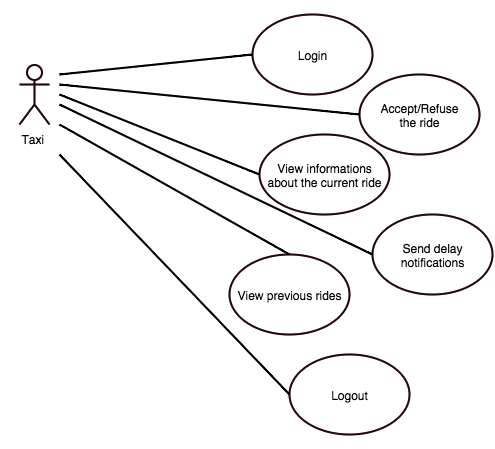
\includegraphics[width=0.70\textwidth]{./images/UseCaseTaxi.png}~
			\end{center}
		
		\subparagraph{Login}
		~\\[0.2cm]
		\vspace{20pt}
		\noindent
		\begin{tabular}{l l}
		 \textbf {Name} & Login  \\ \hline
		 \textbf{Actors} & Taxi \\ \hline
		 \textbf{Entry conditions} & No entry conditions \\ \hline
		 \textbf{Event flow} & 
		 \parbox{0.7\textwidth}{
		 \begin{enumerate}
		 \item The taxi
		    \begin{itemize}
		    \item opens the myTaxiService mobile application;
		    \item clicks on "Log in" link;
		    \item inserts username and password, after the opening of a new window;
		    \item clicks on "Confirm" link;
		    \end{itemize}
		 \item the system accepts the data inserted and the main page is shown to the taxi driver.
		 \end{enumerate}
		 } \\ \hline
		 \textbf{Exit Condition} & No exit conditions \\ \hline
		 \textbf{Exceptions} & \parbox{0.7\textwidth}{If the username and/or the password inserted don't exist in the database, an error message will be shown.}
		\end{tabular}
		
		\newpage
		\subparagraph{Confirmation/Refusal of the service}
		~\\[0.2cm]
		\vspace{20pt}
		\noindent
		\begin{tabular}{l l}
		 \textbf {Name} & Confirm/Refuse the service  \\ \hline
		 \textbf{Actors} & Taxi \\ \hline
		 \textbf{Entry conditions} & Login successful \\ \hline
		 \textbf{Event flow} & 
		 \parbox{0.7\textwidth}{
		 \begin{enumerate}
		 \item The taxi
		 \begin{itemize}
		 \item clicks on the received notification;
		 \item clicks on "Confirm" or "Refuse";
		 \end{itemize}
		 \item the system
		  \begin{itemize}
		 \item sends a notification to the user, if the taxi confirms the service;
		 \item otherwise searches the next available taxi in the queue.
		 \end{itemize}
		 \end{enumerate}
		 } \\ \hline
		 \textbf{Exit Condition} & No exit conditions \\ \hline
		 \textbf{Exceptions} & No exceptions.
		\end{tabular}
		
		\subparagraph{View information about the current ride}
		~\\[0.2cm]
		\vspace{20pt}
		\noindent
		\begin{tabular}{l l}
		 \textbf {Name} & View information about the current ride  \\ \hline
		 \textbf{Actors} & Taxi \\ \hline
		 \textbf{Entry conditions} & Login successful \\ \hline
		 \textbf{Event flow} & 
		 \parbox{0.7\textwidth}{
		 \begin{enumerate}
		 \item The taxi clicks on "View information";
		 \item the system loads from the database the information of the current ride.
		 \end{enumerate}
		 } \\ \hline
		 \textbf{Exit Condition} & No exit conditions \\ \hline
		 \textbf{Exceptions} & No exceptions.
		\end{tabular}
		
		\newpage
		\subparagraph{Send delay notifications}
		~\\[0.2cm]
		\vspace{20pt}
		\noindent
		\begin{tabular}{l l}
		 \textbf {Name} & Send delay notification  \\ \hline
		 \textbf{Actors} & Taxi \\ \hline
		 \textbf{Entry conditions} & Login successful \\ \hline
		 \textbf{Event flow} & 
		 \parbox{0.7\textwidth}{
		 \begin{enumerate}
		 \item The taxi clicks on "Send delay notification";
		 \item the system advises the user about the delay.
		 \end{enumerate}
		 } \\ \hline
		 \textbf{Exit Condition} & No exit conditions \\ \hline
		 \textbf{Exceptions} & No exceptions.
		\end{tabular}
		
		\subparagraph{View previous rides}
		~\\[0.2cm]
		\vspace{20pt}
		\noindent
		\begin{tabular}{l l}
		 \textbf {Name} & View information about the previous rides  \\ \hline
		 \textbf{Actors} & Taxi \\ \hline
		 \textbf{Entry conditions} & Login successful \\ \hline
		 \textbf{Event flow} & 
		 \parbox{0.7\textwidth}{
		 \begin{enumerate}
		 \item The taxi clicks on "View history";
		 \item the system loads from the database the information of all the previous rides.
		 \end{enumerate}
		 } \\ \hline
		 \textbf{Exit Condition} & No exit conditions \\ \hline
		 \textbf{Exceptions} & No exceptions.
		\end{tabular}
		
		\subparagraph{Where is the user?}
		~\\[0.2cm]
		\vspace{20pt}
		\noindent
		\begin{tabular}{l l}
		 \textbf {Name} & Where is the user?  \\ \hline
		 \textbf{Actors} & Taxi \\ \hline
		 \textbf{Entry conditions} & Login successful \\ \hline
		 \textbf{Event flow} & 
		 \parbox{0.7\textwidth}{
		 \begin{enumerate}
		 \item The taxi clicks on the button "Where is the user?";
		 \item the system sends an SMS to the user to tell him/her that the taxi is arrived.
		 \end{enumerate}
		 } \\ \hline
		 \textbf{Exit Condition} & No exit conditions \\ \hline
		 \textbf{Exceptions} & No exceptions.
		\end{tabular}
		\newpage
		\subsubsection{Sequence Diagrams}
	Some sequence diagrams of the system's most interesting aspects
	\begin{center}
		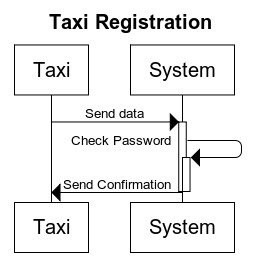
\includegraphics[width=0.60\textwidth]{./images/Taxi_Registration}
	\end{center}
	In order to register a taxi must send his identifier and a password to the system that localize him using the gps and inserts him into the appropriate queue. After this the system confirms the registration.
		\newpage
	\begin{center}
		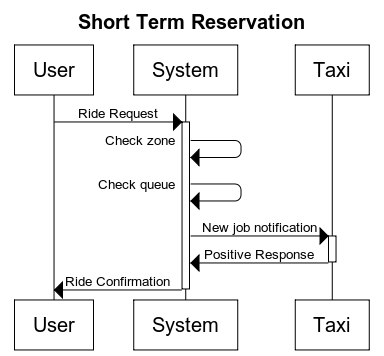
\includegraphics[width=0.80\textwidth]{./images/Short_Term_Reservation}
	\end{center}
	In order to request a short term reservation ride a user must send his address; date and hours must be omitted in this case. The system check where the address is located and the queue associated to that zone; then sends a notification to the first taxi in the queue and after the taxi confirmation, the system confirms the reservation to the user.
		\newpage
	\begin{center}
		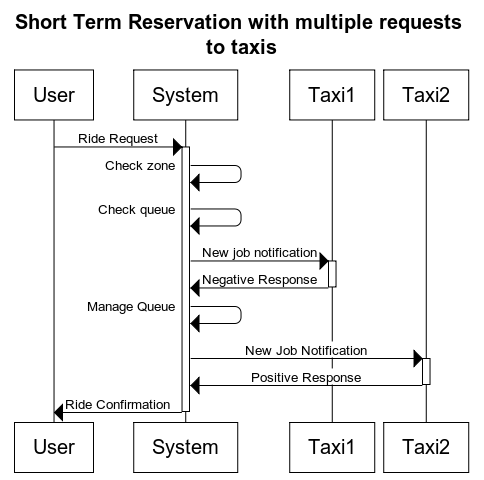
\includegraphics[width=0.90\textwidth]{./images/Short_Term_Reservation_with_multiple_requests_to_taxis}
	\end{center}
	In order to request a short term reservation ride a user must send his address; date and hours must be omitted in this case. The system check where the address is located and the queue associated to that zone; then sends a notification to the first taxi in the queue and since the first taxi answers with a negative response the system puts the taxi at the end of the queue and asks to the second taxi in the queue. After the taxi confirmation, the system confirms the reservation to the user.
		\newpage
	\begin{center}
		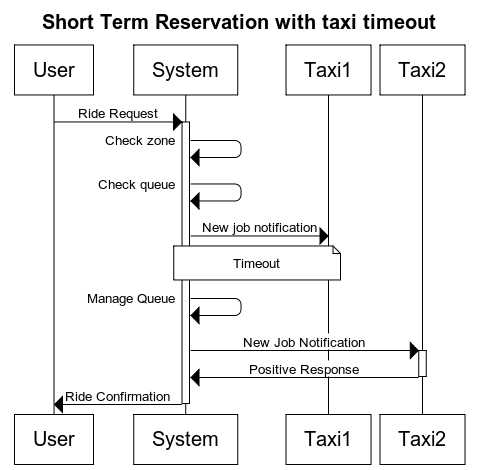
\includegraphics[width=0.90\textwidth]{./images/Short_Term_Reservation_with_taxi_timeout}
	\end{center}
	In order to request a short term reservation ride a user must send his address; date and hours must be omitted in this case. The system check where the address is located and the queue associated to that zone; then sends a notification to the first taxi in the queue and since the first taxi doesn't answers the system, after a timeout, puts the taxi at the end of the queue and asks to the second taxi in the queue. After the taxi confirmation, the system confirms the reservation to the user.
		\newpage
	\begin{center}
		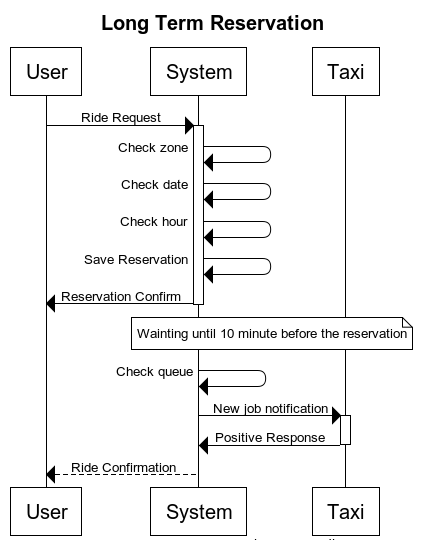
\includegraphics[width=0.90\textwidth]{./images/Long_Term_Reservation}
	\end{center}
	In order to request a long term reservation ride a user must send his address, the date and the hours of the reservation. Te system check where the address is located and stores the reservation i the database and confirms the user his reservation. Ten minutes before the ride the system check the queue associated with the address zone and send a notification to the taxi. After the positive answer by the taxi the system confirms the user his ride.

		\newpage
		\subsubsection{Class Diagram}
\begin{center}

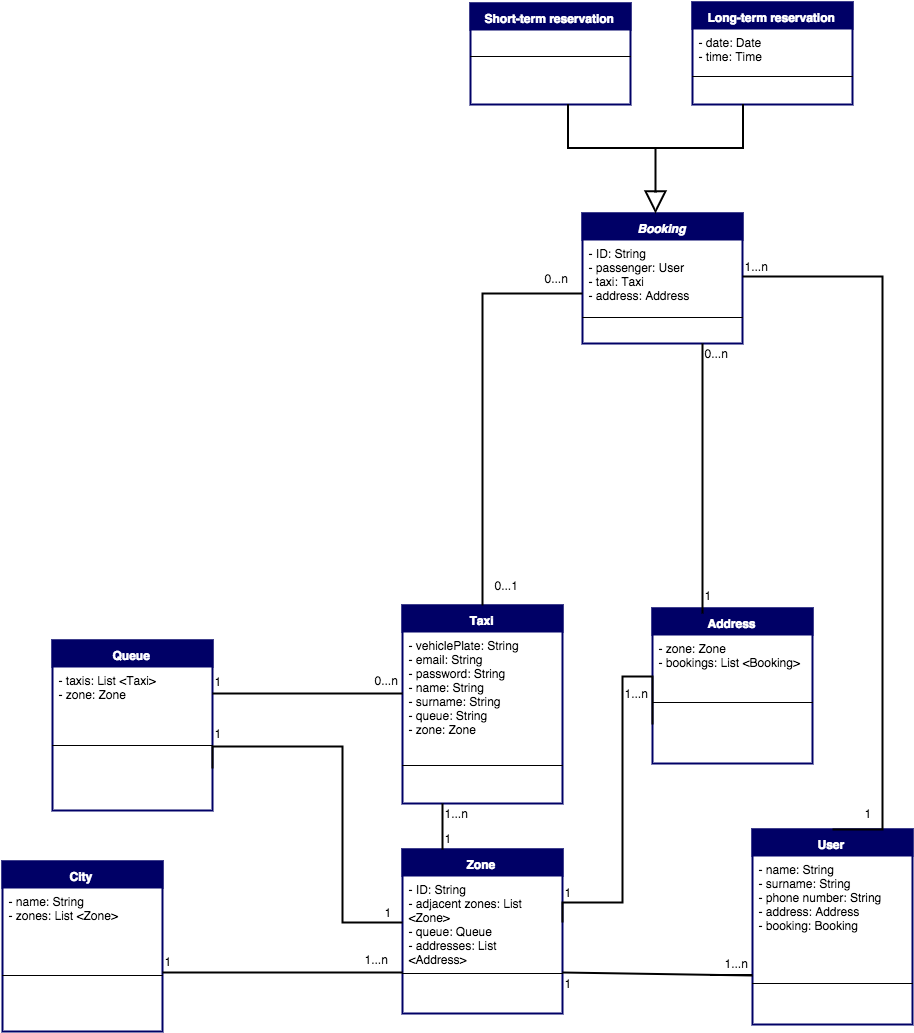
\includegraphics[width=0.95\textwidth]{./images/ClassDiagram.png}
	\end{center}
	
Starting from the definition of the "City" class, we are been able to define the other classes, specifying the relations between them. Only the class "Booking" is an abstract one and it is extended by two other classes, "Short-term Reservation" and "Long-term Reservation".
We are written for the classes some private attributes, that are relevant, in our opinion. These attributes connect a class to another, with reference to the relations, defined before. 
We have omitted the classes methods because this Class Diagram lets us to have a first overview and because we will not implement this system.
		\newpage
\subsection{Alloy}
	\subsubsection{Signatures}
		\lstinputlisting{myTaxiService_signatures.txt}
\newpage
	\subsubsection{Facts}
		\lstinputlisting{myTaxiService_facts.txt}
	\subsection{Assertions}
		\lstinputlisting{myTaxiService_assertions.txt}
	\subsection{Non-Functional Requirements}
		\begin{itemize}
		\item The system will provide a secure access to their personal page for all the taxi drivers, using a username and a password.
		\item In case of long-term reservation, the user must book a taxi at least two hours before the meeting time.
		\item In case of long-term reservation modification or elimination, the user must do it at least 15 minutes before the meeting time.
	    \item The system will be used the GPS information to locate the taxis position.
	    \item If a taxi doesn't answer to a service notification in at most 5 minutes, the system moves it at the end of the queue and it sends a notification to the new first available taxi of that queue. 
		\end{itemize}
